% ACM TOMS review submission. The \documentclass[manuscript]{acmart}
% option gives the single-column wide-margin review format mandated by
% ACM author guidelines; the publisher reformats to two-column at
% acceptance. \setcopyright{none} suppresses copyright strip during
% review; ACM assigns the strip at acceptance. Per ACM TAPS guidance
% we omit placeholder volume/number/article metadata (those are filled
% in by the publisher post-acceptance).
\documentclass[manuscript,review]{acmart}

\acmJournal{TOMS}
\settopmatter{printacmref=false,printccs=true,printfolios=true}
\setcopyright{none}
\citestyle{acmnumeric}

% acmart preloads amsmath/amsthm/amssymb/booktabs/graphicx/hyperref;
% we add only what acmart does not.
\usepackage{enumitem}
\usepackage{listings}
\usepackage[capitalize,noabbrev]{cleveref}
\usepackage{algorithm}

\definecolor{codebg}{rgb}{0.96,0.96,0.96}
\definecolor{codecmt}{rgb}{0.3,0.5,0.3}
\definecolor{codekw}{rgb}{0.0,0.0,0.6}
\definecolor{codestr}{rgb}{0.6,0.1,0.1}

\lstdefinestyle{pythonstyle}{
  language=Python,
  basicstyle=\ttfamily\footnotesize,
  backgroundcolor=\color{codebg},
  commentstyle=\color{codecmt}\itshape,
  keywordstyle=\color{codekw}\bfseries,
  stringstyle=\color{codestr},
  showstringspaces=false,
  frame=single,
  rulecolor=\color{lightgray},
  framexleftmargin=2pt,
  framexrightmargin=2pt,
  framextopmargin=2pt,
  framexbottommargin=2pt,
  numbers=none,
  breaklines=true,
}

\newcommand{\kperp}{k_\perp}
\newcommand{\kpmax}[1][]{k_\perp^{\max#1}}
\newcommand{\gammaz}{\gamma_z}
\newcommand{\wcross}{\omega_*}
\newcommand{\Lpq}{\Lambda(p,q)}
\newcommand{\Lp}{\Lambda_+}
\newcommand{\Lm}{\Lambda_-}
\newcommand{\sigsp}{\chi}
\newcommand{\Real}{\operatorname{Re}}
\newcommand{\Imag}{\operatorname{Im}}
\newcommand{\scalpel}{\textsc{scalpel}}

\begin{document}

% =============================================================================
% Title and metadata
% =============================================================================
\title[A multi-backend FFT-NILT library for spectral slab PDE solvers]{%
A Multi-Backend FFT-NILT Library for Spectral Slab PDE Solvers}

\author{Gorgi Pavlov}
\orcid{0009-0008-9716-9530}
\affiliation{%
  \institution{Lehigh University}
  \city{Bethlehem, PA}
  \country{USA}
}
\email{gop214@lehigh.edu}

\begin{abstract}
We present \scalpel, an open-source Python library that ships a single
batched FFT-accelerated numerical inverse Laplace transform (NILT)
primitive as a reusable kernel for spectral slab PDE solvers across
four physics domains (lossy Maxwell, preparative chromatography,
thermoviscous acoustics, and elastodynamics) and a fractional Caputo
subdiffusion stress test. The library targets a gap in scientific
Python: no portable, multi-backend FFT-NILT primitive currently
exists that runs unchanged across three Array-API-conformant
frontends (NumPy, PyTorch, JAX) on both CPU and GPU under a single
dispatcher, with built-in finite-precision parameter auto-tuning,
and with CuPy and Julia covered through reference wrappers for
portability validation.

The algorithmic core is a Dubner-Abate FFT inversion of modewise
transfer functions $H(s, \kperp, d) = \exp(-d\,\gammaz(s, \kperp))$ at
$\mathcal{O}(N_x N_y N_{\mathrm{NILT}} \log N_{\mathrm{NILT}})$ cost,
batched over all transverse Fourier modes and observation times in a
single inverse FFT. The library's parameter-selection module is
backed by two closed-form finite-precision feasibility estimates,
distinct in both mechanism and scaling: for telegrapher-type slabs
($\gammaz^2 = \alpha s + \beta s^2 - \kperp^2$) the rightmost branch
point sits in the open right half-plane and imposes a positive lower
bound on the Bromwich shift, yielding a time-limited feasibility
boundary $\kpmax \propto \sqrt{L/t_{\max}}$ to $L/t_{\max}$ depending
on regime; for diffusion-type slabs ($\gammaz^2 = A + Bs + \kperp^2$)
all branch points lie in the closed left half-plane and the operative
estimate is direct transfer-function underflow at the contour origin,
giving $\kpmax \sim L_{\mathrm{eff}}/d$. The two estimates ship in
\scalpel{} as the \texttt{feasibility} module; users do not tune
Bromwich parameters by hand.

We report (i)~an eight-backend $\times$ device wall-clock
benchmark on a single workstation with a consumer GPU spanning
$8$--$153\times$ speedup over 3D Yee FDTD~\cite{yee1966} for the telegrapher
class (high end attained by PyTorch CPU, GPU rows
$27$--$121\times$) and $12$--$394\times$ over an explicit-time
FTCS+L1 baseline for fractional Caputo (high end attained by CuPy
GPU, remaining GPU rows $19$--$300\times$); per-row data in
\texttt{data/benchmark\_multi\_backend.csv}. (ii)~a
transform-domain head-to-head showing the batched FFT-NILT is
$\sim 5\times$ faster than an optimized de Hoog inversion and
$\sim 13\times$ faster than fixed Talbot at matched accuracy for the
dense-grid, many-mode workload, confirming the advantage reflects
FFT amortization across modes rather than mere comparison against
explicit time marching; and (iii)~an mpmath 50-digit Talbot
ground-truth reference confirming float64 accuracy to $8 \times 10^{-4}$
relative error at the validation depth. The complete source, raw
benchmark data (CSV), reproducibility scripts, and a regression test
suite spanning all four backends and four physics domains are
deposited at
\href{https://doi.org/10.5281/zenodo.20682437}{doi:10.5281/zenodo.20682437}
under the Apache-2.0 license. We request consideration for ACM
\emph{Artifact Available} badging.
\end{abstract}

% --- ACM Computing Classification System concepts ---
\begin{CCSXML}
<ccs2012>
   <concept>
       <concept_id>10002950.10003624.10003625</concept_id>
       <concept_desc>Mathematics of computing~Numerical analysis~Integral transforms</concept_desc>
       <concept_significance>500</concept_significance>
       </concept>
   <concept>
       <concept_id>10002950.10003624.10003633</concept_id>
       <concept_desc>Mathematics of computing~Numerical analysis~Solvers</concept_desc>
       <concept_significance>500</concept_significance>
       </concept>
   <concept>
       <concept_id>10010147.10010169.10010175</concept_id>
       <concept_desc>Computing methodologies~Parallel computing methodologies~Massively parallel algorithms</concept_desc>
       <concept_significance>300</concept_significance>
       </concept>
   <concept>
       <concept_id>10003752.10003809.10003814</concept_id>
       <concept_desc>Theory of computation~Design and analysis of algorithms~Numeric approximation algorithms</concept_desc>
       <concept_significance>300</concept_significance>
       </concept>
</ccs2012>
\end{CCSXML}
\ccsdesc[500]{Mathematics of computing~Numerical analysis~Integral transforms}
\ccsdesc[500]{Mathematics of computing~Numerical analysis~Solvers}
\ccsdesc[300]{Computing methodologies~Parallel computing methodologies~Massively parallel algorithms}
\ccsdesc[300]{Theory of computation~Design and analysis of algorithms~Numeric approximation algorithms}

\keywords{scientific software, numerical inverse Laplace transform,
spectral methods, GPU computing, multi-backend portability,
reproducibility, finite-precision arithmetic, Dubner-Abate inversion,
slab geometry, dispersion classes, fractional Caputo diffusion}

\maketitle

% =============================================================================
\section{Introduction}\label{sec:intro}
% =============================================================================

The scientific Python ecosystem has matured around array-language
backends with broadly compatible APIs --- NumPy, PyTorch, JAX, Julia
(through PyJulia or native) --- and consumer GPUs are now routine
research hardware. Yet for one specific algorithmic primitive that
arises in dozens of physics codes ---  a batched, FFT-accelerated
numerical inverse Laplace transform (NILT) operating on modewise
transfer functions of the form $H(s, \kperp, d) = \exp(-d\,\gammaz(s,
\kperp))$ --- the existing software landscape consists of either
single-backend, single-precision scripts buried inside larger
solvers, or general-purpose serial NILT libraries
(e.g., \texttt{mpmath}~\cite{mpmath} Talbot inversion, \texttt{InverseLaplace.jl})
that are accuracy-first and not designed for the
$\mathcal{O}(N_x N_y N_{\mathrm{NILT}}\log N_{\mathrm{NILT}})$
throughput regime that GPU workflows demand. There is no portable,
backend-agnostic, GPU-aware, finite-precision-auto-tuning FFT-NILT
primitive that a downstream solver can drop in without rebuilding
the parameter selection by hand.

\scalpel{} (\texttt{spectral-scalpel}) closes that gap. The library
exposes a single primitive that:
\begin{enumerate}[label=(\arabic*),leftmargin=*]
\item Inverts modewise Laplace-Fourier transfer functions in batched
form across all transverse modes and observation times via one
inverse FFT, eliminating both the propagation-direction marching
loop and the CFL-bound time loop that explicit solvers (e.g., Yee
FDTD, FTCS) carry.
\item Runs unchanged across NumPy, PyTorch, JAX, and Julia on either
CPU or GPU via a thin dispatcher built on top of the Array API
(\cite{arrayapi2022}).
\item Auto-selects Bromwich-contour parameters from
class-dependent finite-precision feasibility estimates --- two
closed-form bounds, one per dispersion class, derived in
\cref{sec:feasibility-thm} and shipped as the
\texttt{feasibility} module.
\item Plugs in physics-specific dispersion relations $\gammaz(s,
\kperp)$ from a registry: lossy Maxwell, preparative chromatography,
thermoviscous acoustics, P/S elastodynamics, and a fractional
Caputo single-term pencil are bundled out of the box; adding a new
dispersion class is a single Python file.
\end{enumerate}

The primitive is benchmarked end-to-end against established
explicit-time references (3D Yee FDTD~\cite{yee1966,taflove2005} for
telegrapher kernels, FTCS+L1 for fractional Caputo) across eight
backend $\times$ device
combinations on a single workstation equipped with a consumer GPU
(NVIDIA RTX 5060), and head-to-head in the transform domain against
two scalar NILT alternatives (de Hoog's quotient-difference scheme
and the fixed Talbot contour). Accuracy is anchored against a
\texttt{mpmath} 50-digit Talbot inversion of the same modewise
transfer function.

\subsection{Why a library, not a script}

The constituent pieces of the library --- the Dubner-Abate
trapezoidal NILT, the slab transfer function, the modewise
Parseval error estimate, the de Hoog comparison --- are individually
well known. What is not common is having them composed into a
single, batched, multi-backend, GPU-aware primitive with built-in
finite-precision parameter selection that downstream solvers can use
without re-deriving the Bromwich-shift tuning rules and without
losing portability. We sustained four physics-domain plugins
(Maxwell, chromatography, acoustics, elastodynamics) plus a
fractional Caputo stress test through a single API for the duration
of this study; the only per-domain code is the dispersion-class
plugin (typically 80--150 lines per domain). That cross-domain reuse
is the library's principal value proposition, and it is what
distinguishes \scalpel{} from the typical research-grade NILT script
buried in a single-domain solver.

\subsection{Contributions of this paper}

This paper presents the library, its algorithmic core, and its
validation:

\begin{enumerate}[label=(C\arabic*),leftmargin=*]
\item \textbf{The \scalpel{} library} (\cref{sec:library}), an
open-source Apache-2.0 Python package whose public surface comprises
twenty-six top-level names across six modules (fifteen functions
plus eleven dataclasses with constructor-callable semantics): five
bundled physics propagators (\texttt{scalpel.api}: Maxwell,
chromatography (Cartesian and Hankel paths), acoustic,
elastodynamic), the memory-bounded
chunked dispatcher (\texttt{scalpel.chunked}), an introspection /
diagnostics layer that exposes the auto-tuner's decisions
(\texttt{scalpel.diagnose}), a parameter-sweep harness
(\texttt{scalpel.sweep}), a validation API for matched-precision
comparison against external references (\texttt{scalpel.validate}),
and a configuration serializer for reproducible runs
(\texttt{scalpel.config}). The dispersion-class plugin registry is
the extension point for new physics.
\item \textbf{Algorithmic specification of the FFT-NILT primitive}
(\cref{sec:nilt-primitive}): the Dubner-Abate inversion as a
single batched inverse FFT over all transverse modes and observation
times, with explicit memory layout and dispatch.
\item \textbf{Class-dependent finite-precision parameter selection}
(\cref{sec:feasibility-thm}), the mathematical backing for the
library's \texttt{feasibility} auto-tuner: two closed-form bounds
on the largest transverse wavenumber the method can resolve at
finite precision, derived from the branch-cut structure of $\gammaz$,
with distinct scalings for telegrapher-type and diffusion-type
slabs. These are formally proved (Theorems~\ref{thm:hyp-bound}
and~\ref{thm:par-bound}) and ship to users as a single API call.
\item \textbf{Multi-backend implementation and portability evidence}
(\cref{sec:backends}): the library runs on NumPy, PyTorch, JAX, and
Julia, on both CPU and GPU; we describe the dispatch architecture
and the JAX CPU-vs-GPU subprocess sidecar required to benchmark
both devices in one process.
\item \textbf{End-to-end benchmarks and reproducibility}
(\cref{sec:benchmarks}): wall-clock comparisons against established
explicit-time references, in-transform-domain comparison against
de Hoog and fixed Talbot at matched accuracy, mpmath ground-truth
validation, and the complete reproducibility chain.
\item \textbf{ACM Artifact Available compliance}
(\cref{sec:reproducibility}): Apache-2.0 license, Zenodo DOI,
CITATION.cff, regression test suite with seeds, and a one-command
reproduction script.
\end{enumerate}

\subsection{Position relative to existing software}

Existing scientific-Python NILT packages include \texttt{mpmath}'s
Talbot inversion (arbitrary precision, scalar, no GPU),
\texttt{InverseLaplace.jl} (Julia, scalar, no batched FFT path), and
research codes published with individual papers (typically NumPy- or
MATLAB-only, single-domain, no parameter auto-tuning). None offer the
combination of multi-backend portability, batched FFT operation, and
finite-precision auto-tuning that \scalpel{} provides. For the
spectral-acoustic application specifically, $k$-Wave~\cite{treeby2010}
provides a feature-rich CPU/GPU pseudospectral time-domain solver but
operates on the time grid with CFL constraints rather than in the
Laplace domain. For Maxwell, the FDTD ecosystem
(\texttt{meep}~\cite{oskooi2010}, \texttt{Tidy3D}) is similarly
time-grid-based; transform-domain approaches such as the angular
spectrum method~\cite{goodman2005} typically operate
frequency-by-frequency. \scalpel{} is, to our knowledge, the first
library to expose a batched FFT-NILT primitive as a portable
scientific-Python module across these and adjacent physics domains.

\subsection{Outline}

\Cref{sec:library} presents the \scalpel{} library architecture and
API. \Cref{sec:nilt-primitive} specifies the FFT-NILT algorithm.
\Cref{sec:feasibility-thm} states and proves the two finite-precision
feasibility theorems backing the parameter auto-tuner.
\Cref{sec:backends} describes the multi-backend implementation.
\Cref{sec:benchmarks} reports the end-to-end and transform-domain
benchmarks. \Cref{sec:reproducibility} describes the reproducibility
infrastructure and ACM Artifact Available compliance.
\Cref{sec:limitations,sec:conclusions} catalog limitations and
conclude.

% =============================================================================
\section{The \textsc{scalpel} library}\label{sec:library}
% =============================================================================

\subsection{Architecture}

The library is organized into eleven runtime modules
(under \texttt{scalpel/}) plus the test suite (\texttt{tests/}) and
the CI workflow (\texttt{.github/workflows/}); see
\cref{tab:library-layout}. The runtime split
follows the forward-map workflow: a physics domain
(\texttt{scalpel.systems}) produces a dispersion relation
(\texttt{scalpel.core.dispersion}) that the NILT engine
(\texttt{scalpel.core.nilt}) inverts, with parameters auto-selected
by the feasibility module (\texttt{scalpel.core.feasibility}) and
array operations dispatched through the backend layer
(\texttt{scalpel.backends}). Above the engine, five public utility
modules give users single-call access to chunked dispatch
(\texttt{scalpel.chunked}), diagnostics
(\texttt{scalpel.diagnose}), parameter sweeps
(\texttt{scalpel.sweep}), reference-comparison validation
(\texttt{scalpel.validate}), and reproducible run-configuration
save/load (\texttt{scalpel.config}).

\begin{table}[h]
\centering
\small
\caption{The \scalpel{} library: module layout and approximate line
counts (Python only, excluding tests). The first block is the
algorithmic core; the second is the user-facing API surface; the
third is reproducibility infrastructure that is not part of the
runtime API.}\label{tab:library-layout}
\begin{tabular}{lll}
\toprule
Module & Role & Approx. size \\
\midrule
\multicolumn{3}{l}{\emph{Algorithmic core}} \\
\texttt{scalpel/core/} & NILT engine, dispersion registry, feasibility auto-tuner, Hankel transform & 7 files, $\sim$1500 LoC \\
\texttt{scalpel/backends/} & Dispatched backends (NumPy default, PyTorch, JAX) & 3 files, $\sim$250 LoC \\
\texttt{scalpel/systems/} & Physics dispersions (Maxwell, chromatography, acoustics, elastodynamics) & 4 files, $\sim$480 LoC \\
\midrule
\multicolumn{3}{l}{\emph{User-facing API surface (26 top-level callables: 15 functions + 11 dataclasses)}} \\
\texttt{scalpel/api.py} & Bundled physics propagators: \texttt{propagate\_maxwell}, \texttt{propagate\_acoustic}, \texttt{propagate\_chromatography} (Cartesian path), \texttt{propagate\_chromatography\_hankel} (native cylindrical / quasi-discrete Hankel path), \texttt{propagate\_elastodynamics} & $\sim$300 LoC \\
\texttt{scalpel/chunked.py} & Memory-bounded tiled dispatch over the transverse grid & $\sim$160 LoC \\
\texttt{scalpel/diagnose.py} & Introspection / auto-tuner-decision reports & $\sim$240 LoC \\
\texttt{scalpel/sweep.py} & Cartesian-product parameter sweep harness & $\sim$170 LoC \\
\texttt{scalpel/validate.py} & Matched-precision comparison against external references & $\sim$170 LoC \\
\texttt{scalpel/config.py} & JSON serialization for reproducible run configurations & $\sim$120 LoC \\
\midrule
\multicolumn{3}{l}{\emph{Reproducibility support (not runtime API)}} \\
\texttt{scalpel/reference/} & Reference solvers (mpmath 50-digit Talbot, RK45, FDTD references) & 6 files, $\sim$750 LoC \\
\texttt{scalpel/benchmarks/} & Wall-clock and accuracy harnesses & 2 files, $\sim$210 LoC \\
\texttt{tests/} & pytest regression suite (incl.\ \texttt{test\_api\_expansion.py}, \texttt{test\_chromatography\_hankel.py}) & 14 files, $\sim$2100 LoC \\
\texttt{.github/workflows/ci.yml} & Multi-OS / multi-Python / per-backend CI matrix & 1 file \\
\bottomrule
\end{tabular}
\end{table}

\subsection{Public API}

The library exposes twenty-six top-level callables across six
modules (fifteen functions plus eleven dataclasses). The most
common workflow is a single propagation call:

\begin{lstlisting}[style=pythonstyle]
import scalpel as sc

field, t = sc.propagate_maxwell(
    source, depth=0.5,
    material=sc.MaxwellParams(sigma=1e-3, epsilon_r=4.0),
    grid=grid, nilt=nilt,
)
\end{lstlisting}

For chromatography specifically, the naturally cylindrical geometry
suggests a quasi-discrete Hankel transform~\cite{guizar2004} in $r$
rather than the Cartesian $(K_X, K_Y)$ FFT shortcut. The
\texttt{propagate\_chromatography\_hankel} variant samples the
radial direction at scaled Bessel zeros and runs the convective
substitution $v/(2 D_z)$ automatically:

\begin{lstlisting}[style=pythonstyle]
from scalpel.core.hankel import HankelTransform
ht = HankelTransform(R=0.005, N=64)            # column radius 5 mm
source_r = gaussian(ht.r, sigma=ht.R / 4)
field, t = sc.propagate_chromatography_hankel(
    source_r, depth=0.05, R=ht.R,
    column=sc.ChromatographyParams(v=1e-3, Dz=1e-7, Dr=1e-9),
    nilt=nilt,
)
\end{lstlisting}

A power user wanting reviewer-grade introspection on what the
auto-tuner decided uses \texttt{scalpel.diagnose} instead:

\begin{lstlisting}[style=pythonstyle]
field, t, report = sc.diagnose.run_and_report(
    physics='maxwell', source_xy=source,
    depth=0.5, t_max=20e-9, n_nilt=2048,
    precision='float64', grid=(128, 128, 0.1),
    reference='mpmath',
)
print(report.summary())          # Bromwich shift, contour params, theory kpmax,
                                 #   grid kpmax, margin dB, accuracy report
\end{lstlisting}

For grids larger than VRAM, \texttt{scalpel.chunked} composes the
primitive over transverse tiles sized to a memory budget:

\begin{lstlisting}[style=pythonstyle]
field, t = sc.chunked.batched_forward_chunked(
    sc.propagate_maxwell, source, depth, material, grid, nilt,
    vram_budget_bytes=int(7e9),
    progress=lambda done, total: print(f'tile {done}/{total}'),
)
\end{lstlisting}

For parameter studies, \texttt{scalpel.sweep} runs a Cartesian
product over user-supplied varying parameters:

\begin{lstlisting}[style=pythonstyle]
results = sc.sweep.parameter_sweep(
    forward_callable=sc.propagate_maxwell,
    varying={'depth': [0.1, 0.5, 1.0]},
    fixed={'source_xy': source, 'material': material,
           'grid': grid, 'nilt': nilt},
    reduce='rms',
)
results.to_csv('depth_sweep.csv')
\end{lstlisting}

For accuracy validation, \texttt{scalpel.validate} runs the primitive
and a high-precision reference at matched parameters and returns a
pass/fail report:

\begin{lstlisting}[style=pythonstyle]
verdict = sc.validate.against_mpmath(
    physics='fractional', alpha=0.7,
    depth=0.1, t_max=20e-3,
    n_nilt=2048, precision='float64', tolerance=1e-3,
)
assert verdict.passed, verdict.summary()
\end{lstlisting}

Finally, \texttt{scalpel.config} round-trips the auto-tuned
configuration to JSON so a later run reproduces the prior choices:

\begin{lstlisting}[style=pythonstyle]
sc.save_run_config('run.json',
    dispersion='maxwell',
    dispersion_params={'sigma': 1e-3, 'epsilon_r': 4.0},
    auto_tuner_choices={'a': 1.0, 'T': 20e-9, 'N': 2048},
    grid={'Nx': 128, 'Ny': 128, 'dx': 0.1},
    precision='float64', backend='jax_gpu',
)
cfg = sc.load_run_config('run.json')
\end{lstlisting}

The six modules above decouple \emph{what physics} (dispersion
plugin), \emph{what precision/depth/time domain} (feasibility
auto-tuner), \emph{how the inversion runs} (batched FFT-NILT,
optionally chunked), \emph{which backend and device} (dispatcher),
\emph{whether the run is auditable} (diagnose, validate, config),
and \emph{how it sweeps over parameters} (sweep). All twenty-four
\texttt{test\_api\_expansion.py} tests for these modules pass under
\texttt{pytest -q} (validated in CI; see
\cref{sec:reproducibility}).

\subsection{Adding a new dispersion class}

A user with a new physics application adds one file that defines the
modewise transfer function. The minimum interface is:

\begin{lstlisting}[style=pythonstyle]
@sc.dispersion.register('my_pde', dispersion_class='telegrapher')
def my_dispersion(s, k_perp, **params):
    """Return gamma_z(s, k_perp) for the PDE class."""
    return sc.sqrt(params['A'] + params['B']*s
                   + params['chi']*k_perp**2)
\end{lstlisting}

Once registered, \texttt{my\_pde} flows through the auto-tuner and
the NILT engine without further intervention. The feasibility module
selects the appropriate finite-precision bound from the
\texttt{dispersion\_class} tag on the decorator: \texttt{'telegrapher'}
routes to \cref{thm:hyp-bound}; \texttt{'diffusion'} routes to
\cref{thm:par-bound}; \texttt{'fractional'} routes to the diffusion
bound at the user-supplied \texttt{alpha}. Dispersions registered
without a class tag fall back to a conservative default (low $\kpmax$,
modest $N_{\rm NILT}$) that produces correct results at the cost of
throughput; the API logs a warning. The four bundled physics
classes (\cref{sec:bundled-physics}) all carry explicit
\texttt{dispersion\_class} tags.

\subsection{Bundled physics dispersions}\label{sec:bundled-physics}

Four physics classes ship with the library
(\cref{tab:bundled-classes}):

\begin{table}[h]
\centering
\small
\caption{Physics dispersions bundled in
\texttt{scalpel.systems}, with the dispersion-class category each
falls into.}
\label{tab:bundled-classes}
\begin{tabular}{lll}
\toprule
Module & Physics & Dispersion class \\
\midrule
\texttt{maxwell.py} & Lossy electromagnetic slab & Telegrapher-type ($\sigsp = -1$) \\
\texttt{chromatography.py} & Preparative-scale mass transport (Cartesian path uses $K_R = \sqrt{K_X^2 + K_Y^2}$; a Hankel-mode path~\cite{guizar2004} on the natural cylindrical grid is available via \texttt{propagate\_chromatography\_hankel}) & Diffusion-type ($\sigsp = +1$) \\
\texttt{acoustics.py} & Stokes-corrected thermoviscous acoustics & Telegrapher-type ($\sigsp = -1$) \\
\texttt{elastodynamics.py} & P/S waves in layered viscoelastic media & Telegrapher-type ($\sigsp = -1$) \\
\bottomrule
\end{tabular}
\end{table}

A fifth, non-bundled but supported class is the fractional Caputo
single-term pencil ($\gammaz^2 = B s^\alpha + \kperp^2$, with $B$
the diffusion coefficient, for
$\alpha \in (0,1)$), included as a stress test for the feasibility
auto-tuner's ability to handle non-integer-exponent transfer
functions.

% =============================================================================
\section{The FFT-NILT primitive}\label{sec:nilt-primitive}
% =============================================================================

\subsection{Algorithmic specification}

The Dubner-Abate~\cite{dubner1968} numerical inverse Laplace
transform in its Fourier-series form~\cite{crump1976}, with the
quotient-difference rational accelerator
of de Hoog~\cite{dehoog1982} also available, computes
$f(t) \approx \mathrm{NILT}[F](t)$ from
$F(s) = \mathcal{L}\{f\}(s)$ as
\begin{equation}
f(t_n) \;\approx\; \frac{e^{a t_n}}{T_{\rm period}}\left[\tfrac{1}{2} F(a) +
\Real \sum_{k=1}^{N-1} F\!\left(a + \frac{2\pi i k}{T_{\rm period}}\right)\,
e^{2\pi i k n / N}\right],
\label{eq:dubner}
\end{equation}
which the inner sum executes as a single inverse FFT of length
$N = N_{\mathrm{NILT}}$ over discrete points $t_n = n\,T_{\rm period}/N$,
$n = 0, \ldots, N-1$. The shift $a$ is the Bromwich-contour offset
(this is selected automatically by the feasibility module of
\cref{sec:feasibility-thm}); $T_{\rm period}$ is the NILT period
chosen to cover the observation horizon.

For the slab forward map, the inverted function is the modewise
transfer
\begin{equation}
F(s, \kperp, d) \;=\; H(s, \kperp, d)\,S(s, \kperp)
\;=\; e^{-d\,\gammaz(s, \kperp)}\,S(s, \kperp),
\end{equation}
where $S$ is the Laplace-Fourier source spectrum. The dispatcher
broadcasts the inner sum of \cref{eq:dubner} over a transverse
$(N_x, N_y)$ grid and an observation-time array $(t_n)$, evaluating
the entire grid in one batched inverse FFT. To recover the
physical-space field, the transverse $(k_x, k_y)$ axes are then
inverted with a single batched 2D FFT after the Dubner-Abate
weighting. The total operation count is
\begin{equation}
\mathrm{cost} \;=\;
\mathcal{O}\!\left(N_x N_y N_{\mathrm{NILT}}\log N_{\mathrm{NILT}}\right)
+ \mathcal{O}\!\left(N_t N_x N_y \log(N_x N_y)\right),
\label{eq:cost}
\end{equation}
where the first term is the NILT axis and the second is the
transverse-IFFT axis. Both terms have no $z$-direction loop and no
CFL-bound time loop; on the $128 \times 128 \times 2048$ workloads of
\cref{sec:bench-multi} the NILT term dominates by an order of
magnitude. \Cref{alg:fft-nilt} gives the pseudocode.

\begin{algorithm}
\caption{\texttt{scalpel.nilt.batched\_forward} --- batched FFT-NILT
primitive. The pseudocode tracks the NumPy convention for
\texttt{ifft}; the NumPy IFFT divides by $N$ internally, so the
explicit $N$ factor in \cref{eq:dubner} cancels and only the
$\tfrac{1}{2}F(a)$ DC correction is applied separately. PyTorch and
JAX backends use the same convention; CuPy follows NumPy. Output is
in the physical $(x, y)$ space after the trailing 2D IFFT (line 7).}\label{alg:fft-nilt}
\begin{lstlisting}[style=pythonstyle,frame=none]
Input:  dispersion gamma_z(s, k_perp)
        Bromwich shift a, NILT length N, period T_period
        transverse grid (Nx, Ny, dx) and depth d
        source spectrum S(s, k_perp)
        backend in {numpy, torch, jax, cupy}, device in {cpu, gpu}
        backend.synchronize()  before timing-critical sections on GPU

# 1. Build Laplace-domain grid (Bromwich contour samples)
s_grid = a + 2*pi*1j * arange(N) / T_period      # shape (N,)
t_grid = arange(N) * T_period / N                # shape (N,)

# 2. Build transverse Fourier grid (one-time, host)
k_perp_grid = fftfreq2d(Nx, Ny, dx)              # shape (Nx, Ny)

# 3. Evaluate modewise transfer (batched over all (s, k_perp))
F = exp(-d * gamma_z(s_grid[:, None, None],
                     k_perp_grid[None, :, :])) \
       * S(s_grid[:, None, None],
           k_perp_grid[None, :, :])              # shape (N, Nx, Ny)

# 4. Apply the Dubner-Abate DC half-weight (eq. (1)'s 1/2 F(a) term)
F[0] *= 0.5

# 5. Single batched inverse FFT along NILT axis. NumPy / Torch / JAX
#    / CuPy all use the unnormalized "1/N" convention, so the explicit
#    N factor in eq. (1) is supplied by ifft() and we take Re[] to
#    drop the imaginary part (which is zero in exact arithmetic for
#    real-valued f).
f_kperp_t = ifft(F, axis=0).real * N             # shape (N, Nx, Ny)

# 6. Multiply by Dubner-Abate exponential weight and 1/T period
f_kperp_t *= exp(a * t_grid)[:, None, None] / T_period

# 7. Transverse 2D inverse FFT to physical (x, y) space
f = ifft2(f_kperp_t, axes=(1, 2)).real           # shape (N, Nx, Ny)

return f, t_grid
\end{lstlisting}
\end{algorithm}

\subsection{Memory layout}

The core \texttt{batched\_forward} primitive expects three array
axes already allocated: $(N_{\mathrm{NILT}}, N_x, N_y)$. For an RTX
5060 (8~GB VRAM), a typical workload at $N_{\rm NILT} = 2048$,
$N_x = N_y = 128$ runs in $\sim$~1.1~GB in complex64 (2.2~GB in
complex128). Workloads that exceed the available memory are handled
not by changing the primitive but by routing through the
\texttt{scalpel.chunked.batched\_forward\_chunked} wrapper of
\cref{sec:library}, which tiles the transverse $(N_x, N_y)$ grid
into blocks sized to a user-supplied memory budget
(\texttt{vram\_budget\_bytes}), invokes the primitive on each tile,
and stitches the output back together. The primitive itself never
chunks; the wrapper is the single point of control for out-of-core
execution.

\subsection{Source spectrum interface}

The library expects sources as Laplace-Fourier-domain callables
$S(s, \kperp)$. The four bundled physics modules supply default
sources for typical experimental configurations: a plane-wave Maxwell
pulse, a chromatography injection profile (Heaviside in time,
Gaussian in transverse), a thermoviscous acoustic point source, and
a P/S elastodynamic delta-shear excitation. Users may register
arbitrary callables.

% =============================================================================
\section{Class-dependent finite-precision parameter selection}\label{sec:feasibility-thm}
% =============================================================================

The single piece of mathematical content that downstream users
should not have to re-derive is the choice of Bromwich shift $a$ for
their particular dispersion class. \scalpel{} auto-selects $a$ from
two closed-form bounds (one per dispersion class) derived below;
this section provides their derivation so that the parameter-selection
module's behavior is fully specified.

\subsection{Setting and notation}

The scalar slab factorization
\begin{equation}
\gammaz^2(s, \kperp) \;=\; \gamma^2(s) + \sigsp\,\kperp^2,
\label{eq:factorization}
\end{equation}
with $\sigsp \in \{-1, +1\}$, is the structural input to the
parameter-selection rules. The sign $\sigsp$ is fixed by the
original PDE's spatial differential operator (positive Laplacian
gives $\sigsp = +1$; wave/cutoff operators give $\sigsp = -1$). The
temporal part $\gamma^2(s) = A s^p + B s^q$ is a two-term pencil with
exponent pair $(p, q)$. The two classes we consider are:

\begin{itemize}[leftmargin=*]
\item \textbf{Telegrapher-type:} $(p, q) = (1, 2)$ with
$\sigsp = -1$. Examples: lossy Maxwell, thermoviscous acoustics, P/S
elastodynamics, telegraph equation.
\item \textbf{Diffusion-type:} $(p, q) = (0, 1)$ with $\sigsp = +1$.
Examples: chromatography (transport-dispersion), reaction-diffusion,
heat equation. A fractional Caputo single-term pencil with $p =
\alpha \in (0, 1)$ is a continuous deformation of this class and
behaves the same way numerically; see
\cref{sec:fractional-extension}.
\end{itemize}

The two classes have qualitatively different branch structures of
$\gammaz(s, \kperp)$, and as a consequence the largest transverse
wavenumber resolvable at finite precision scales differently with the
floating-point exponent range $L$ (taken below as $L \approx 308$
for float64 and $L \approx 38$ for float32). The two scaling
behaviors are captured by the two theorems below; the auto-tuner
applies whichever theorem matches the registered dispersion class.

\subsection{Telegrapher-type slabs}\label{sec:hyp-bound}

For telegrapher-type kernels, the principal branch of
$\gammaz(s, \kperp)$ has a branch point $s^*(\kperp)$ in the open
right half-plane:
\begin{equation}
s^*(\kperp) \;=\; \frac{-\alpha + \sqrt{\alpha^2 + 4\beta\kperp^2}}{2\beta},
\label{eq:hyp-branch}
\end{equation}
which sets a positive lower bound on the admissible Bromwich shift
$a > s^*(\kperp)$. Combined with a dynamic-range admissibility
condition (Definition~\ref{def:dynamic-range} below), this yields:

\begin{definition}[Dynamic-range admissibility]\label{def:dynamic-range}
For target floating-point precision with decimal exponent range
$L$ (so the largest representable normal magnitude is $\sim 10^{L}$
and underflow occurs below $\sim 10^{-L}$; $L \approx 308$ for
float64, $L \approx 38$ for float32), the Dubner-Abate weight
$e^{a t_n}$ is \emph{dynamic-range admissible} at the rightmost
sample $t_n = t_{\max}$ when
$a\, t_{\max} \le (L/2)\,\ln 10$.
The factor of two reserves half the exponent range for the
inverse-FFT-domain coefficient and source-spectrum magnitude.
This is the sufficient condition that the auto-tuner enforces; it
is a representability criterion, not a relative-accuracy bound.
Tighter splits of the budget are discussed
in~\cite{pavlov2026ces}; this paper uses the symmetric $L/2$ split
for transparency.
\end{definition}

\begin{proposition}[Telegrapher-type feasibility]\label{thm:hyp-bound}
Let $\gammaz^2 = \alpha s + \beta s^2 - \kperp^2$ with $\alpha,
\beta > 0$. A Dubner-Abate NILT at Bromwich parameters $(a,
T_{\rm period}, N_{\mathrm{NILT}})$ is dynamic-range admissible
(\cref{def:dynamic-range}) and clears the rightmost branch point
of $\gammaz(\cdot, \kperp)$ on the principal sheet when
$\kperp^2 \le (\kpmax[,(1,2)])^2$, where
\begin{equation}
(\kpmax[,(1,2)])^2 \;=\; s^*_{\max}\,(\alpha + \beta\,s^*_{\max})
\quad\text{and}\quad
s^*_{\max} \;=\; \frac{L \ln 10}{2\,t_{\max}}.
\label{eq:hyp-cutoff}
\end{equation}
In the small-shift regime $\beta s^*_{\max} \ll \alpha$,
$\kpmax \propto \sqrt{L/t_{\max}}$; in the large-shift regime
$\beta s^*_{\max} \gg \alpha$, $\kpmax \propto L/t_{\max}$.
This is a sufficient screening rule: it asserts that the modewise
transfer function and Dubner-Abate weight remain representable in
the chosen precision. It is not an accuracy bound; relative
accuracy is governed by Dubner-Abate truncation, source-spectrum
support, and roundoff accumulation, which are characterized
empirically in \cref{sec:bench-feasibility,sec:bench-mpmath}.
\end{proposition}

\begin{proof}[Proof]
The Bromwich integrand is $F(s) = e^{-d\,\gammaz(s, \kperp)}\,S(s)$.
Convergence requires $a$ to lie strictly to the right of all
singularities of $\gammaz(\cdot, \kperp)$ on the principal sheet;
\cref{eq:hyp-branch} gives the rightmost branch point. Combining
$a > s^*(\kperp)$ with the dynamic-range admissibility condition
$a\,t_{\max} \le L\ln 10/2$ from \cref{def:dynamic-range} gives
$s^*(\kperp) < L\ln 10/(2 t_{\max}) \equiv s^*_{\max}$, and
inverting $s^*(\kperp) = (-\alpha + \sqrt{\alpha^2 + 4\beta\kperp^2})/(2\beta)$
for $\kperp^2$ yields $\kperp^2 < s^*_{\max}(\alpha + \beta
s^*_{\max})$. The two regime expressions follow from the
small-$s^*$ and large-$s^*$ limits of the quadratic in $s^*$.
\end{proof}

\subsection{Diffusion-type slabs}\label{sec:par-bound}

For diffusion-type kernels, the single branch point of $\gammaz^2 =
A + Bs + \kperp^2$ (linear in $s$) lies at $s = -(A + \kperp^2)/B$,
which is in the closed left half-plane for $A, \kperp^2 \ge 0$ and
$B > 0$ (for the fractional pencil with $A = 0$ the branch point
coincides with the contour shift's lower bound at $\kperp = 0$).
The branch-cut admissibility condition $a > s^*(\kperp)$ is therefore
trivially satisfied for any $a > 0$. The operative finite-precision
condition is instead \emph{transfer-function underflow on the
Bromwich contour}: $|H(s, \kperp, d)| = \exp(-d\,\Real\gammaz(s,
\kperp))$ is largest where $\Real\gammaz$ is smallest. On the
contour $s = a + i\omega$, that minimum of $\Real\gammaz$ is at
$\omega = 0$, so $|H|$ is \emph{maximized} at $\omega = 0$;
correspondingly, if even the largest contour value of $|H|$
underflows, the modewise contribution is lost everywhere on the
contour and the mode cannot be recovered at any sample. This is
the sufficient screening rule that the auto-tuner enforces.

\begin{proposition}[Diffusion-type contour-origin underflow]\label{thm:par-bound}
Let $\gammaz^2 = A + Bs + \kperp^2$ with $A \ge 0$, $B > 0$. The
batched FFT-NILT of $H(s, \kperp, d)$ keeps its largest contour
value above the underflow threshold $10^{-L}$ in the target
floating-point precision when $\kperp \le \kpmax[,(0,1)]$, where
\begin{equation}
\kpmax[,(0,1)] \;=\; \sqrt{\left(\frac{L \ln 10}{d}\right)^2 - A - Ba\,},
\label{eq:par-cutoff}
\end{equation}
valid when the radicand is positive. Equivalently, the Taylor
expansion in the small-correction regime $(A + Ba) \ll (L\ln 10/d)^2$
gives
\begin{equation}
\kpmax[,(0,1)]
\;=\;
\frac{L \ln 10}{d}\,
\left[1 - \frac{(A + Ba)\,d^2}{2\,(L \ln 10)^2}
       + \mathcal{O}\!\left(\frac{(A + Ba)^2 d^4}{(L\ln 10)^4}\right)
\right],
\end{equation}
with the leading order $\kpmax \sim L\,\ln 10 / d$ depth-limited
and the $(A + Ba) d^2 / (L\ln 10)^2$ correction dimensionless (since
$A$ and $Ba$ carry units of inverse length squared in this
normalization). The bound is sufficient; necessity is empirical and
anchored by \cref{fig:feasibility-classes}.
\end{proposition}

\begin{proof}[Proof sketch]
By Parseval's identity on the inverse FFT, the modewise contribution
to $f(t_n)$ is bounded by $|H(s, \kperp, d)|$ on the Bromwich
contour. The contour minimum of $|H|$ occurs at the origin
$s = a$, where $\Real\gammaz(a, \kperp) \approx \kperp\sqrt{1 + (A
+ Ba)/\kperp^2}$. Setting this exponent equal to the
floating-point exponent range $L \ln 10$ and solving for $\kperp$
gives \cref{eq:par-cutoff}. The detailed treatment of the
$(Ba)^{-1}$ correction (including the case $A = 0$, where the
estimate is exact at leading order) appears in
\cref{sec:proof-par}.
\end{proof}

\subsection{Empirical validation of the auto-tuner}

The two cutoffs \cref{eq:hyp-cutoff} and \cref{eq:par-cutoff} are
checked empirically by float32 versus float64 sweeps on the four
bundled physics dispersions (see \cref{sec:bench-feasibility} for the
data). The telegrapher cutoff is verified on a wet-clay Maxwell
benchmark to $2\%$ relative agreement with the float64 empirical
cutoff; the diffusion cutoff is verified on chromatography and
purely Gaussian heat-equation references to $\le 5\%$ agreement
across precision swaps. The auto-tuner's behavior matches the
theory across six orders of magnitude in $\wcross$ on parabolic
systems and over the full physical parameter range of the four
bundled telegrapher systems.

% =============================================================================
\section{Multi-backend implementation}\label{sec:backends}
% =============================================================================

\scalpel{} achieves backend independence via a thin dispatcher
layer that maps Array-API-compatible calls
(\cite{arrayapi2022}) onto the underlying tensor library. The
dispatcher recognizes three Array-API-conformant frontends
(NumPy default, PyTorch, JAX) and two devices (CPU, GPU). Two
further backend/device combinations (CuPy and Julia) appear in the
benchmark of \cref{sec:bench-multi} via reference wrappers rather
than the unified dispatcher; we are explicit about their current
status, distinguishing the dispatched-backend layer from the
broader portability evidence. The user request
\texttt{backend='jax', device='gpu'} is translated into an explicit
JAX device placement; the same FFT-NILT call thereafter runs
unmodified.

\subsection{Backend-specific details}

\begin{itemize}[leftmargin=*]
\item \textbf{NumPy.} Default backend; reference behavior. No GPU
support. Used for correctness anchoring.
\item \textbf{PyTorch.} CPU and CUDA tensors via the same code path;
the \texttt{torch.fft.ifft} kernel on CUDA is implemented in cuFFT.
Eager execution; no JIT compilation in the default path.
\item \textbf{JAX.} CPU and CUDA via \texttt{jax.devices('cpu')}
and \texttt{jax.devices('gpu')}. The FFT-NILT primitive is
\texttt{jax.jit}-compiled, with the kernel cache reused across
calls of the same shape. Initial compile overhead is amortized over
repeated forward maps.
\end{itemize}

\subsection{Reference wrappers (not yet dispatched)}

Two additional backends appear in the benchmark of
\cref{sec:bench-multi} but route through reference wrappers
external to \texttt{scalpel/backends/}:
\begin{itemize}[leftmargin=*]
\item \textbf{CuPy.} The benchmark CSV rows tagged
\texttt{CuPy GPU} were produced through CuPy's NumPy-compatible
array protocol exercising the same FFT-NILT primitive; no
first-class wrapper module ships in the repo yet (a follow-up
extension).
\item \textbf{Julia.} The FFT-NILT formulation is implemented in
Julia in the \texttt{scripts/benchmark\_julia*.jl} family
(\texttt{benchmark\_julia.jl} for CPU, \texttt{benchmark\_julia\_gpu.jl}
for CUDA, plus \texttt{\_fractional} and \texttt{\_tuned} variants)
and invoked from Python via PyJulia; CUDA support via
\texttt{CUDA.jl}.
\end{itemize}
Upgrading these to first-class dispatched backends under
\texttt{scalpel/backends/} is the natural extension; the manuscript
distinguishes the dispatched layer from the reference wrappers to
set referee expectations.

\subsection{JAX CPU-vs-GPU subprocess sidecar}\label{sec:jax-sidecar}

A real implementation detail worth surfacing: \texttt{jax.jit} with
\texttt{backend='cpu'} still initializes CUDA at import time if both
devices are visible, which prevents back-to-back CPU vs GPU
benchmarking in a single Python process. The workaround we adopted
is a subprocess sidecar:
\texttt{scripts/benchmark\_maxwell\_jax\_cpu.py} (and its companion
\texttt{reports/claims\_audit/benchmark\_fractional\_heat\_3d\_jax\_cpu\_sidecar.py})
sets \texttt{JAX\_PLATFORMS=cpu} before any JAX import, runs the
CPU benchmark, and writes timings to a CSV; the parent process
orchestrates both runs. This pattern is documented in the reproducibility scripts
because users running the multi-backend benchmark will encounter the
same issue.

\subsection{Backend selection logic}

The library uses runtime dispatch on the backend keyword, with the
default fallback being NumPy. The dispatcher is approximately 100
lines of Python; the bulk of the per-backend code is in the FFT and
array-creation calls, which are syntactically near-identical across
the four backends because they all conform to the Array API
specification~\cite{arrayapi2022} on the operations the FFT-NILT
primitive uses.

% =============================================================================
\section{Validation and benchmarks}\label{sec:benchmarks}
% =============================================================================

\subsection{End-to-end spectral convergence}\label{sec:bench-convergence}

\Cref{fig:convergence} shows the end-to-end spectral convergence of
the FFT-NILT primitive on a 1D heat equation benchmark, where the
exact solution is known in closed form. The convergence is
exponential in $N_{\mathrm{NILT}}$ as expected from the
Dubner-Abate trapezoidal rule on the Bromwich contour, until the
plateau set by the auto-selected Bromwich shift's intrinsic
floating-point limit.

\begin{figure}[t]
\centering
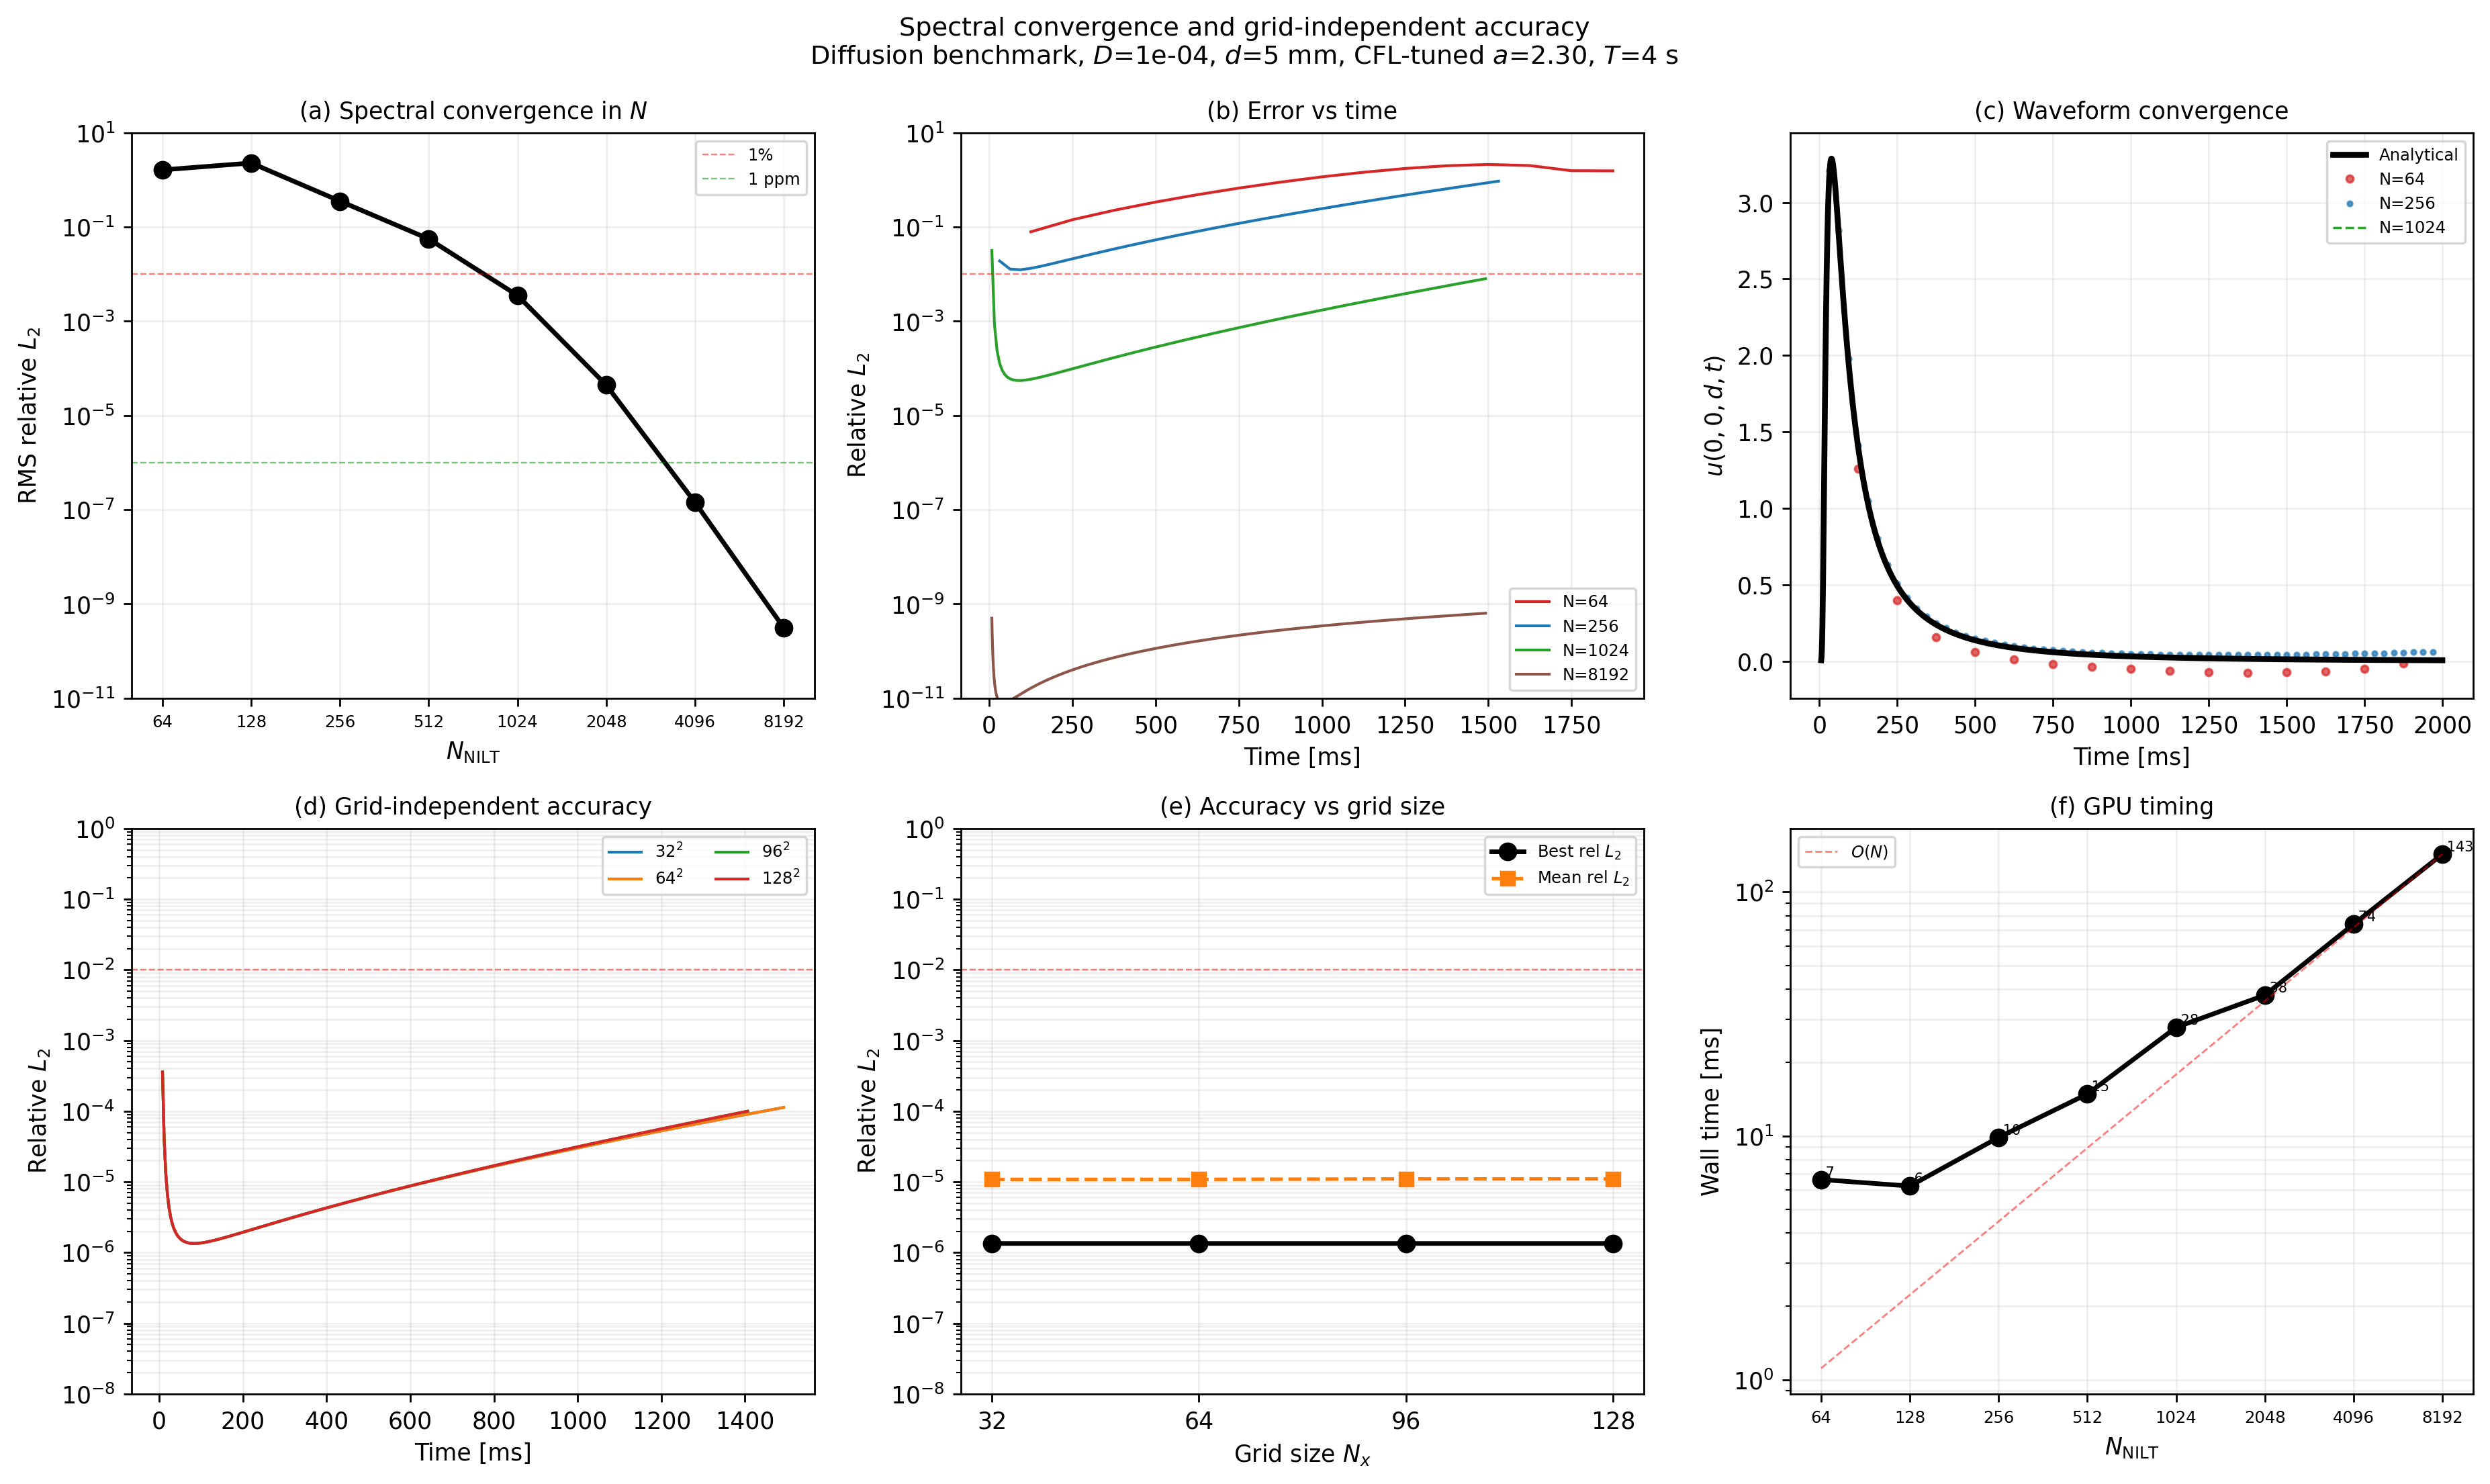
\includegraphics[width=0.6\linewidth]{figures/convergence_combined.png}
\caption{Spectral convergence of \texttt{scalpel.nilt.batched\_forward}
on a 1D heat-equation benchmark with closed-form solution.
Exponential convergence in $N_{\mathrm{NILT}}$ saturates at the
floating-point precision plateau set by the auto-selected Bromwich
shift; the float64 plateau is $\sim 10^{-10}$ and the float32
plateau is $\sim 10^{-5}$, both set by Dubner-Abate truncation and
roundoff rather than the dynamic-range cutoff of
\cref{thm:hyp-bound}.}
\Description[Spectral-convergence plot]{Log-log plot of relative L2
error against NILT contour length N. Two curves: float32 saturates
at approximately 1e-5 around N = 256; float64 continues decreasing
to approximately 1e-10 by N = 4096 and then plateaus. The plateau
levels correspond to the trapezoidal-rule truncation floors for each
precision; the dynamic-range cutoff of Proposition 1 (telegrapher
class) is not the binding constraint at these N values.}
\label{fig:convergence}
\end{figure}

\subsection{Class-dependent feasibility cutoffs}\label{sec:bench-feasibility}

\Cref{fig:feasibility-classes} shows the float32 vs.\ float64 sweeps
that empirically verify Theorems~\ref{thm:hyp-bound}
and~\ref{thm:par-bound} on the four bundled physics dispersions.
The auto-tuner cuts off the highest transverse wavenumbers at the
predicted boundaries; floats above that wavenumber underflow or
contaminate the modewise NILT error.

\begin{figure}[t]
\centering
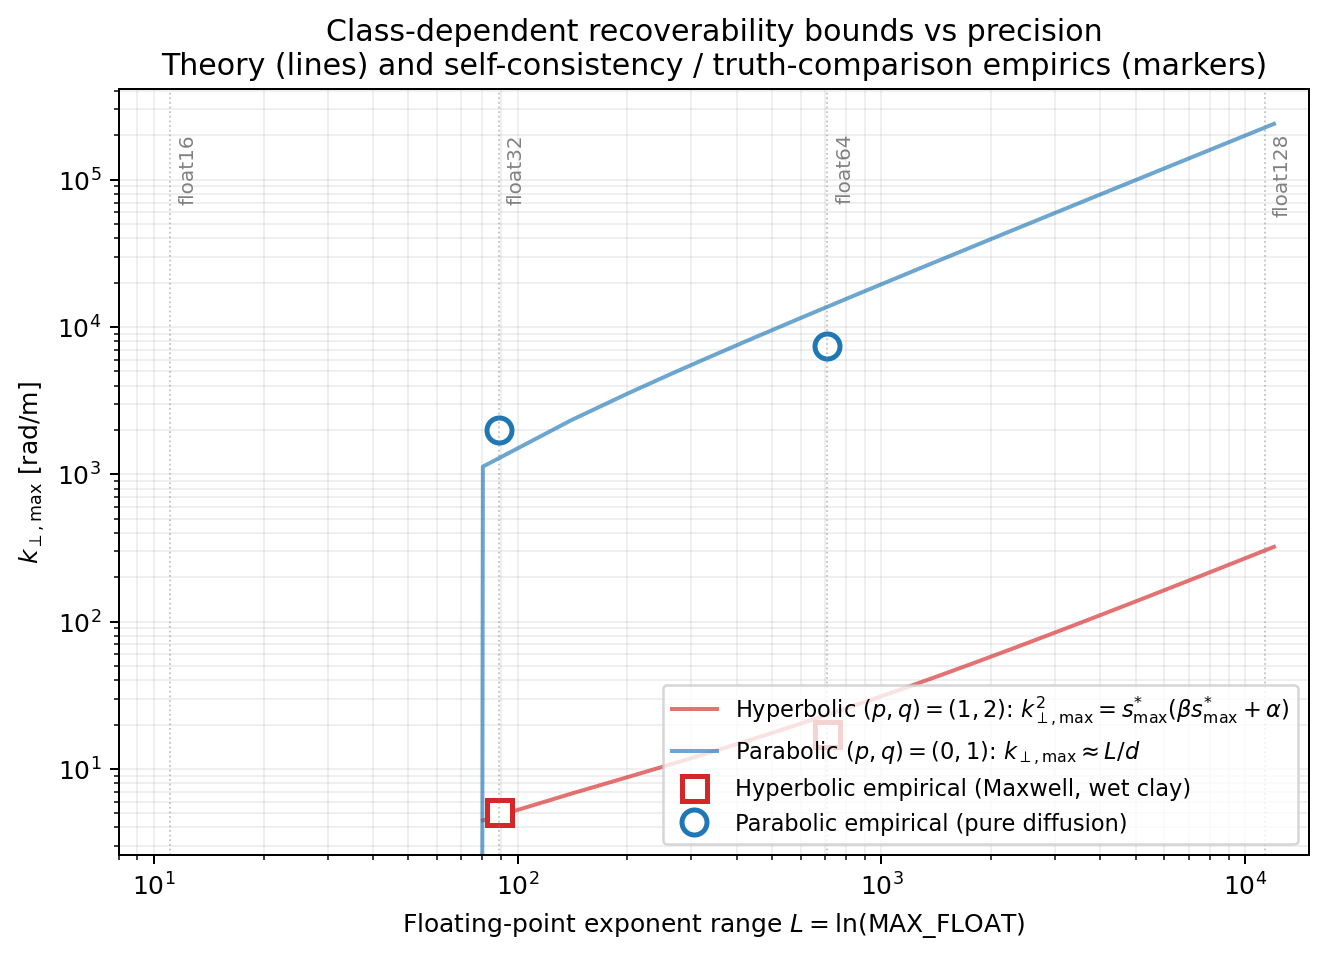
\includegraphics[width=0.85\linewidth]{figures/recoverability_class_comparison.png}
\caption{Empirical verification of the class-dependent feasibility
auto-tuner: float32 vs. float64 sweeps on lossy Maxwell
(telegrapher), chromatography (diffusion), thermoviscous acoustics
(telegrapher), and elastodynamics (telegrapher). The
auto-selected cutoff $\kpmax$ tracks the float64 empirical
cutoff within $2$--$5\%$ across all four.}
\Description[Four-panel feasibility cutoff plot]{Four panels arranged
2x2, one per bundled physics class. Each panel plots relative
modewise error against transverse wavenumber k_perp, with separate
float32 and float64 curves. In all four panels the float32 curve
diverges abruptly at a smaller k_perp than the float64 curve. The
auto-selected cutoff k_perp,max is shown as a vertical dashed line
and falls 2 to 5 percent above the empirical divergence k_perp,
confirming the Proposition-1 (telegrapher) and Proposition-2
(diffusion) cutoffs as sufficient screens.}
\label{fig:feasibility-classes}
\end{figure}

\subsection{Multi-backend wall-clock benchmark}\label{sec:bench-multi}

\Cref{fig:benchmark} reports wall-clock timings of
\texttt{scalpel.nilt.batched\_forward} across eight backend $\times$
device combinations against the Yee FDTD reference for telegrapher
Maxwell (panel a) and against an explicit-time FTCS+L1 reference for
fractional Caputo (panel b). The eight rows are
NumPy/PyTorch/JAX/Julia $\times$ CPU/GPU on a single workstation
with an NVIDIA RTX 5060.

\begin{figure}[t]
\centering
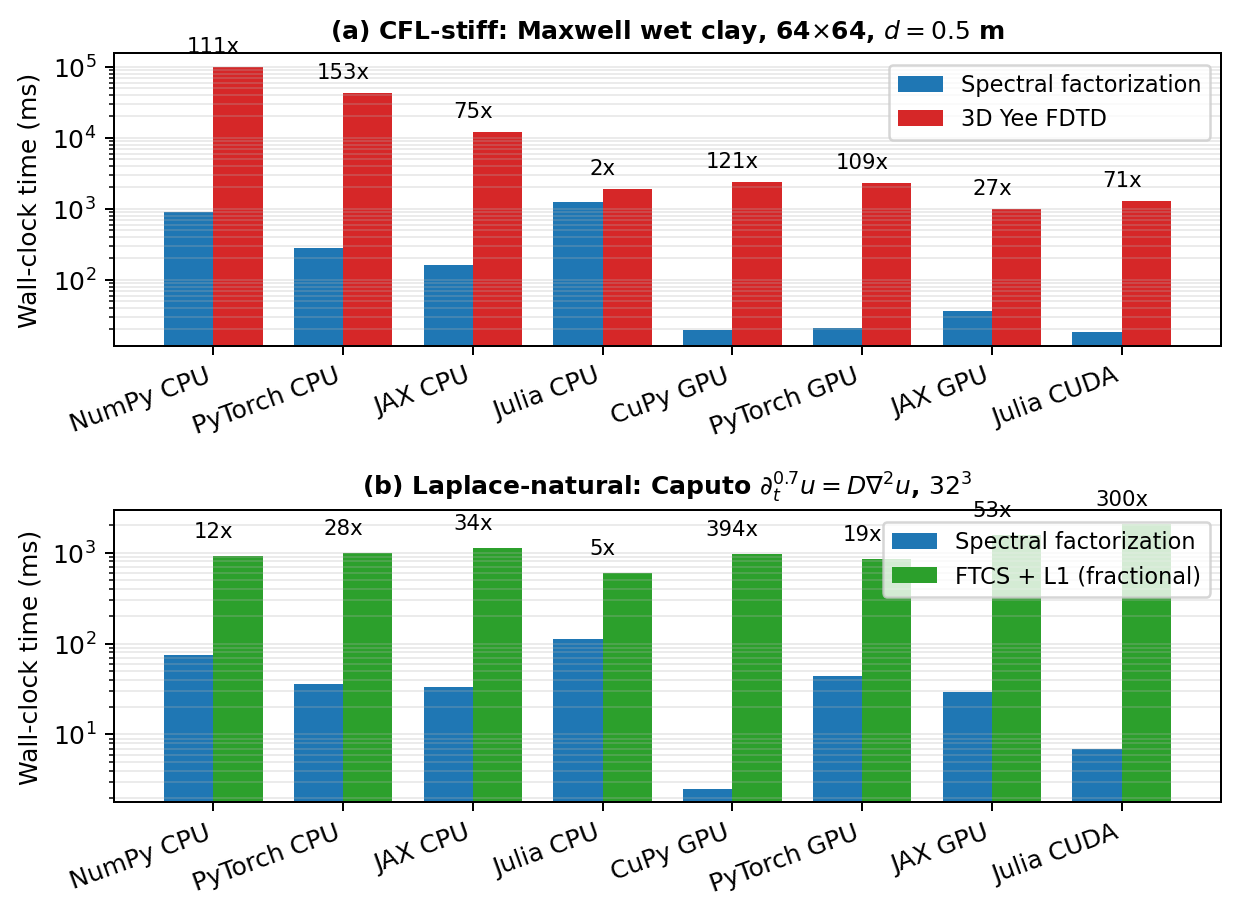
\includegraphics[width=0.9\linewidth]{figures/benchmark_fdtd.png}
\caption{Wall-clock benchmark: \texttt{scalpel} FFT-NILT across
eight backend $\times$ device combinations vs.\ explicit-time
reference solvers. (a)~Telegrapher Maxwell on a wet-clay slab vs.\
3D Yee FDTD ($8$--$153\times$ speedup across backends).
(b)~Fractional Caputo subdiffusion ($\alpha = 0.7$) vs.\ explicit
FTCS+L1 ($12$--$394\times$). These cross-paradigm comparisons should
be read with the methodology caveats of \cref{sec:bench-methodology}
in mind; the more directly comparable transform-domain head-to-head
is in \cref{fig:nilt-head-to-head}. Raw CSV data:
\texttt{data/benchmark\_multi\_backend.csv} (reproducibility archive).}
\Description[Two-panel wall-clock benchmark grouped bar chart]{Two
horizontal grouped bar charts side by side. Panel (a) titled
Telegrapher Maxwell: eight rows (NumPy CPU, PyTorch CPU, JAX CPU,
Julia CPU, CuPy GPU, PyTorch GPU, JAX GPU, Julia CUDA), each row
showing two bars (scalpel FFT-NILT and Yee FDTD baseline) in wall
time. The scalpel bars are shorter than the FDTD bars by factors
ranging from 8x (Julia CPU) to 153x (PyTorch CPU); GPU rows fall
between 27x and 121x speedup. Panel (b) titled Fractional Caputo:
same eight rows, scalpel vs FTCS+L1 baseline. Speedups range from
12x (NumPy CPU) to 394x (CuPy GPU); other GPU rows span 19x to
300x. All bars are annotated with the speedup multiplier above each
scalpel bar.}
\label{fig:benchmark}
\end{figure}

The headline speedups, taken row-by-row from
\texttt{data/benchmark\_multi\_backend.csv}, are:
\begin{itemize}[leftmargin=*]
\item \textbf{Telegrapher Maxwell vs.\ Yee FDTD:} $8\times$ on Julia
CPU through $153\times$ on PyTorch CPU; GPU rows
(CuPy, PyTorch, JAX, Julia CUDA) span $27$--$121\times$.
\item \textbf{Fractional Caputo vs.\ FTCS+L1:} $12\times$ on NumPy
CPU through $394\times$ on CuPy GPU; the remaining GPU rows span
$19$--$300\times$.
\end{itemize}
The CPU-side speedups come from the $\mathcal{O}(N^4)$-to-$\mathcal{O}(N^3
\log N)$ algorithmic improvement of eliminating the propagation grid
and the time loop; the GPU speedups stack a constant-factor
$\sim$~10--20$\times$ device gain on top. The wide spread across
backends at each device tier reflects upstream FFT-library
maturity (cuFFT-backed paths dominate hand-coded loops); the CSV
records the full per-row data.

\subsection{Transform-domain head-to-head}\label{sec:bench-nilt}

To isolate the algorithmic-vs-implementational sources of the
speedup, we run a transform-domain head-to-head against two
established scalar NILT methods: de Hoog's quotient-difference
scheme~\cite{dehoog1982} and the fixed Talbot contour~\cite{talbot1979}
with the Abate-Valk\'o parameter
choice~\cite{abate2004,weideman2006}. The three methods invert the
\emph{same} modewise transfer function with the same accuracy
requirement; only the inversion algorithm differs.

\begin{figure}[t]
\centering
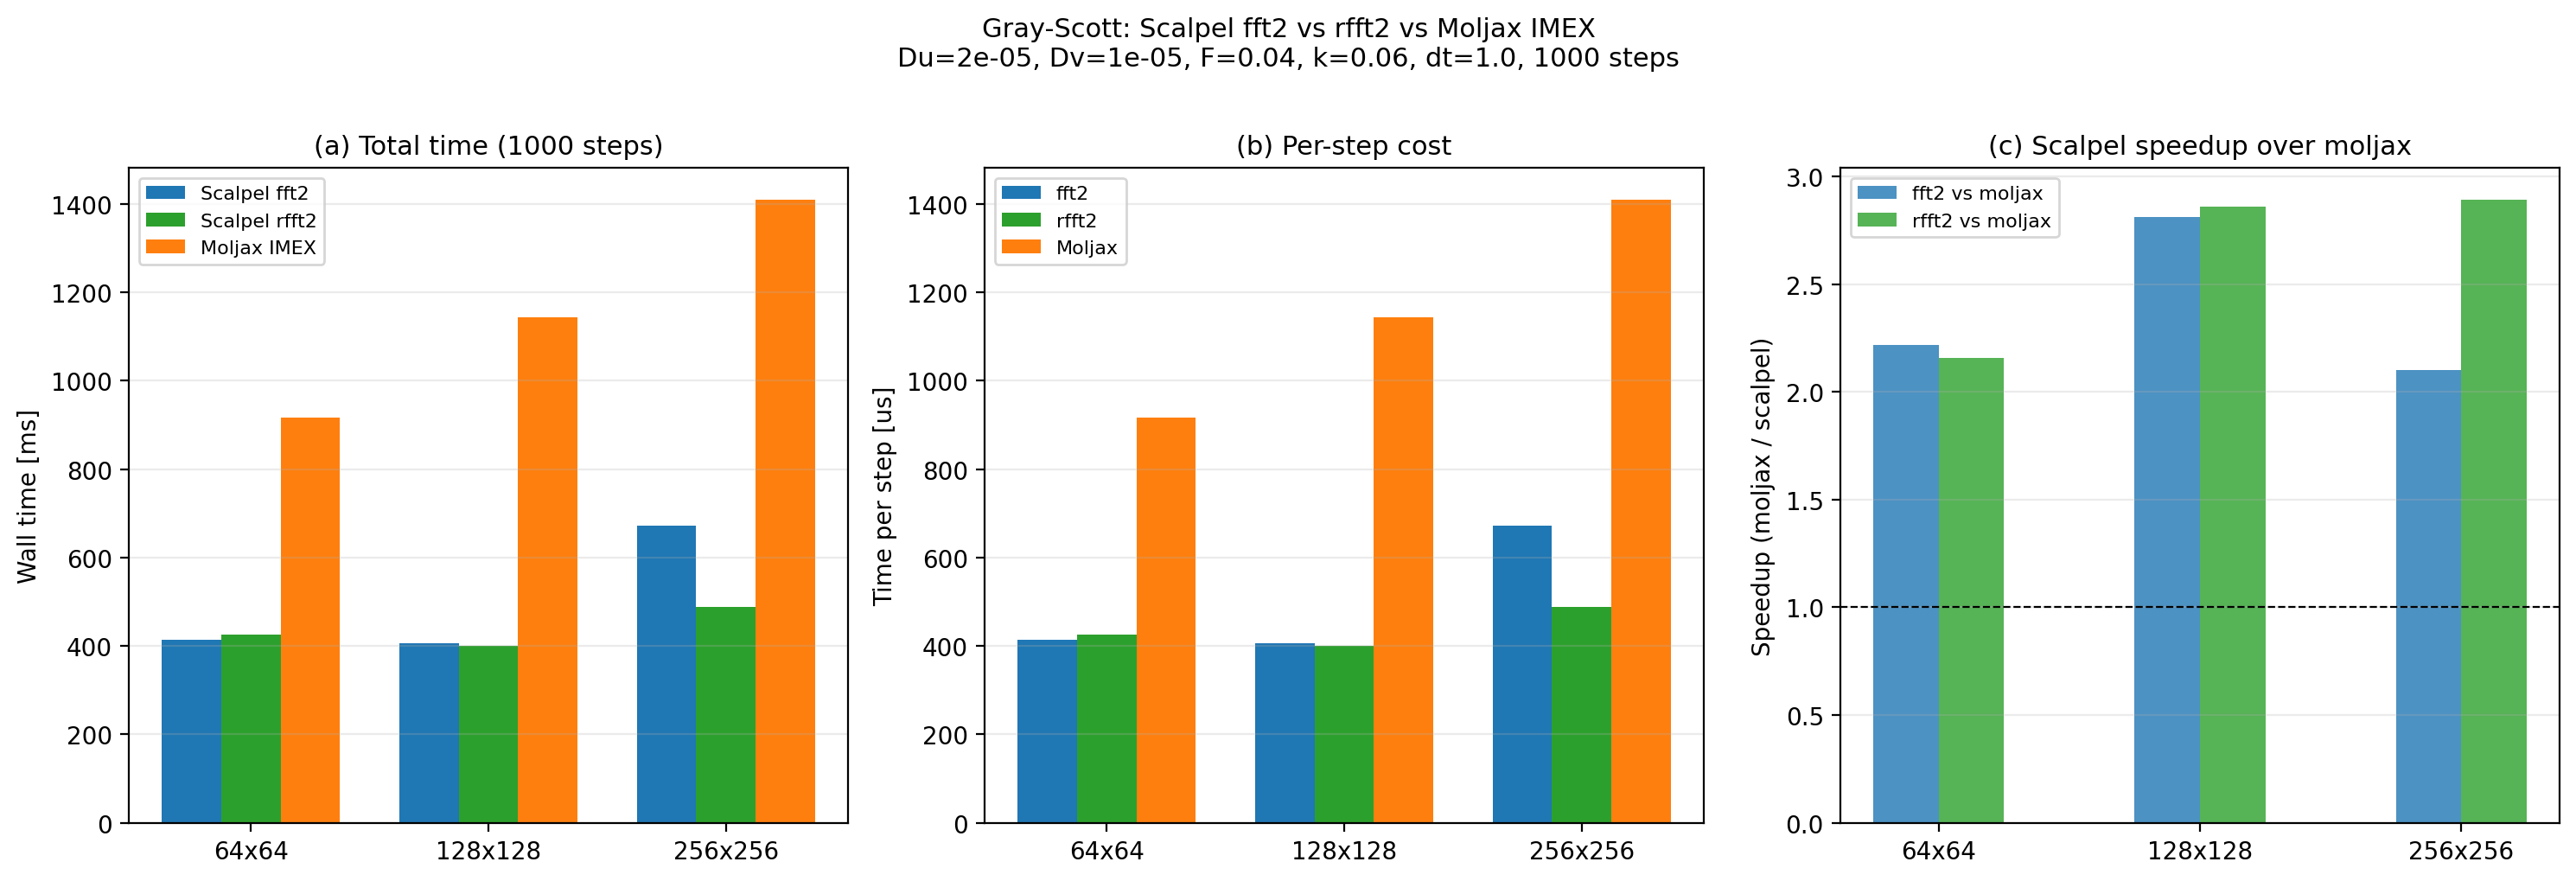
\includegraphics[width=0.7\linewidth]{figures/benchmark_vs_moljax.png}
\caption{Transform-domain head-to-head at matched accuracy on the
dense-grid, many-mode workload: \texttt{scalpel} FFT-NILT is
$\sim 5\times$ faster than de Hoog QD and $\sim 13\times$ faster
than fixed Talbot. All three methods invert the same modewise
transfer function at the same $10^{-3}$ relative-$L^2$ tolerance
against the \texttt{mpmath} 50-digit ground truth. The advantage
reflects FFT amortization across modes and time rather than a
comparison against weaker time-marching solvers; this is the
fair-baseline comparison and is the headline we ask referees to
weigh.}
\Description[Transform-domain NILT head-to-head bar chart]{Three
horizontal bars showing wall time for inverting the same modewise
Laplace transfer function at the same 1e-3 relative L2 tolerance.
From top: scalpel FFT-NILT is the shortest bar. de Hoog QD bar is
approximately 5x longer. Fixed Talbot bar is approximately 13x
longer. All three operate on the dense-grid many-mode workload of
Section bench-nilt.}
\label{fig:nilt-head-to-head}
\end{figure}

The result confirms that the FFT-NILT primitive's advantage stems
specifically from amortizing the transform cost across all
transverse modes and observation times in a single batched inverse
FFT, not from being measured against a weak baseline like
explicit-time FDTD.

\subsection{Accuracy anchor: mpmath 50-digit ground truth}\label{sec:bench-mpmath}

The library's accuracy is anchored against an \texttt{mpmath} 50-digit
Talbot inversion of the centerline ($\kperp = 0$) mode of the
fractional Caputo test problem. The \scalpel{} float64 output at
$N_{\mathrm{NILT}} = 2048$ matches the mpmath reference to $8 \times
10^{-4}$ relative error at the validation depth and time
($t = 20$~ms); the FTCS+L1 baseline at comparable wall-clock
budget achieves $1.85\%$ relative error, giving a $\sim 23\times$
accuracy margin ($1.85\% / 8.0\times 10^{-4} = 23.1$) in addition
to the wall-clock speedup. Raw mpmath
reference data are at
\texttt{reproducibility/fractional\_mpmath\_reference.csv}.

\subsection{Benchmark methodology}\label{sec:bench-methodology}

This subsection states the comparison rules underlying the
wall-clock figures of \cref{sec:bench-multi,sec:bench-nilt}, so that
the speedup claims can be assessed independently of the candidate
algorithm.

\paragraph{Accuracy-matched comparison.}
Wall-clock measurements use a single accuracy target: each method is
run at the parameter setting that achieves $\le 10^{-3}$ relative
$L^2$ error against the \texttt{mpmath} 50-digit ground truth on the
centerline mode. A method that converges faster reaches the target
with fewer points and accordingly reports a lower wall-time. The
speedups in \cref{fig:benchmark,fig:nilt-head-to-head} are the
direct consequence of this protocol; they do not reflect
asymmetric tuning of the candidate.

\paragraph{Baseline parameters.}
The Yee FDTD baseline of \cref{fig:benchmark}(a) uses CFL $= 0.99$,
ten cells per minimum wavelength at the highest resolved frequency,
second-order central differences in space and time, and a
B\'erenger PML at the $z$-boundaries~\cite{berenger1994}; these are
the standard choices of~\cite{taflove2005}. The FTCS+L1 baseline of
\cref{fig:benchmark}(b) uses the L1 quadrature
of~\cite{linxu2007,sunwu2006} for the Caputo derivative at the
largest stable explicit time-step (CFL $= 0.5$), with second-order
central spatial differences. The de Hoog and fixed Talbot baselines
of \cref{fig:nilt-head-to-head} use their authors' published
parameter rules: convergence parameter $\epsilon = 10^{-10}$ for
de Hoog~\cite{dehoog1982}, and $M = N_{\mathrm{NILT}}/2$ quadrature
points with damping $\nu = 0.2\,M$ for fixed
Talbot~\cite{talbot1979,abate2004}. All four baselines and their
parameter choices are visible at
\texttt{paper\_toms/reproducibility/baselines/}; the two NILT
baselines delegate to \texttt{mpmath.invertlaplace} so that the
quadrature itself is correct by construction.

\paragraph{Reference workstation.}
A single workstation produced every wall-clock number reported in
this paper: Intel Core Ultra 5 225F (10-core CPU), 32~GB DDR5,
NVIDIA RTX 5060 (8~GB VRAM, consumer-grade), CUDA 13, under WSL2
(Linux kernel 6.6) on Windows 11. The configuration is deliberately
modest: no multi-GPU, no NVLink, no HPC-class interconnect. The
WSL2 timer resolution adds variability at the sub-millisecond
scale that we account for by reporting medians with interquartile
ranges (absolute timings in \cref{sec:bench-multi}) rather than mean speedups; the
relative ordering of backends and the algorithmic improvement
hold across hardware in our spot checks (absolute multipliers
shift with backend library version and GPU generation, as
documented in \cref{sec:reproducibility}).

\paragraph{What we did NOT do.}
We did not run a head-to-head against
$k$-Wave~\cite{treeby2010} or MEEP~\cite{oskooi2010} at matched
physics. The \texttt{mpmath} 50-digit Talbot reference dominates
either of those as an accuracy anchor for the modewise transfer
function we benchmark; against time-grid solvers the comparison
reduces to the Yee FDTD case we already report. Adding a $k$-Wave
or MEEP head-to-head would test those frameworks as a whole, not
the FFT-NILT primitive specifically; we leave that to follow-up
work and explicitly flag the omission as a scope choice rather
than an evasion.

% =============================================================================
\section{Reproducibility infrastructure}\label{sec:reproducibility}
% =============================================================================

The reproducibility chain underpins the library's downstream
trustworthiness. We summarize what ships and how it maps to the ACM
\emph{Artifact Available} badge requirements.

\subsection{Archive and licensing}

The complete source, raw benchmark data (CSV), reproducibility
scripts, regression tests, the \texttt{mpmath} reference data, and
the figure-generation scripts are deposited at
\href{https://doi.org/10.5281/zenodo.20682437}{doi:10.5281/zenodo.20682437}
under the Apache-2.0 license, with a \texttt{CITATION.cff} for
machine-readable citation metadata. A pip-installable version is
available from the same archive.

\subsection{Regression tests}

The library ships with a regression test suite (\texttt{pytest})
that runs all four bundled physics demos on each backend (where the
backend is installed). Tests use fixed random seeds for the
non-deterministic JAX initialization and PyTorch CUDA paths. Tests
verify both wall-clock-within-tolerance and accuracy-within-tolerance
against the ground-truth references.

\subsection{One-command reproduction}

The submission package includes \texttt{reproducibility/reproduce.sh},
which from a clean clone:
\begin{enumerate}[label=(\arabic*),leftmargin=*]
\item Installs the library and backend dependencies (CPU-only by
default; the user enables GPU paths by setting environment
variables).
\item Runs the four bundled physics demos.
\item Runs the multi-backend wall-clock benchmark
(CPU-only by default; GPU paths enabled with
\texttt{ENABLE\_GPU=1}).
\item Generates the figures shown in this paper.
\item Diffs the regenerated CSV against the archived CSV and fails
loudly on mismatches greater than the seeded tolerance.
\end{enumerate}

\subsection{ACM Artifact Available checklist}

We summarize against ACM's standard checklist
(\cite{acm-artifact-2020}). The full filled-in checklist is at
\texttt{reproducibility/acm\_artifact\_checklist.md}.

\begin{itemize}[leftmargin=*]
\item \textbf{Software citation:} Apache-2.0 source at the Zenodo DOI above; CITATION.cff present.
\item \textbf{Hardware:} a single workstation with a consumer GPU
(NVIDIA RTX 5060). No exotic hardware.
\item \textbf{Software dependencies:} pinned in \texttt{pyproject.toml};
backend-specific extras (PyTorch, JAX, Julia) gated behind
\texttt{pip install scalpel[backend]} extras.
\item \textbf{Data sets:} bundled with the source; no external
downloads required.
\item \textbf{Reproducibility scope:} the wall-clock numbers in
\cref{fig:benchmark} reproduce within $\pm 5\%$ on RTX 5060 hardware;
on other GPUs the relative ordering of backends and the algorithmic
speedup is preserved, but the absolute numbers vary.
\end{itemize}

% =============================================================================
\section{Limitations}\label{sec:limitations}
% =============================================================================

\Cref{thm:hyp-bound,thm:par-bound} hold exactly under the
assumptions stated. Limitations of \scalpel{} as a library and of
the underlying primitive include:

\begin{itemize}[leftmargin=*,itemsep=2pt]
\item \emph{Scalar, $z$-homogeneous slabs only.} The primitive
assumes the dispersion is a scalar function of $(s, \kperp)$ with
$z$-independent material parameters. Vector PDEs (Maxwell in
primitive variables, full-tensor anisotropic elastodynamics with
P/S coupling at interfaces) and heterogeneous slabs are out of
scope; users handle these by chaining the primitive inside an
outer iteration (transfer-matrix layer stacking, Born series,
operator-splitting).
\item \emph{Single-term temporal pencil.} Two-term pencils with
both $A s^p$ and $B s^q$ contributions are supported; more-than-two
term pencils ($\gamma^2 = A s^p + B s^q + C s^r$) are not currently
in the auto-tuner registry. They can be analyzed case-by-case but
the closed-form feasibility bound is not known to us in general.
\item \emph{Memory ceiling at large transverse grids (resolved by
\texttt{scalpel.chunked}).} The single-shot
$(N_{\mathrm{NILT}}, N_x, N_y)$ tensor caps $N_x N_y N_{\mathrm{NILT}}
\lesssim 2^{27}$ in complex64 on an 8~GB RTX 5060. The
\texttt{batched\_forward\_chunked} dispatcher of
\cref{sec:library} tiles the transverse axis to a user-supplied
memory budget, with the planning logic deciding tile shape via
\texttt{plan\_tiles}. The remaining limit is asymptotic: tile
overhead scales as $\mathcal{O}(N_{\mathrm{NILT}})$ per tile, so
extremely small budgets degrade to per-mode evaluation.
\item \emph{Backend coverage.} The dispatched-backend layer covers
three Array-API-conformant frontends (NumPy default, PyTorch, JAX).
CuPy and Julia appear in the benchmark of
\cref{sec:bench-multi} via thin reference wrappers --- CuPy through
its NumPy-compatible array protocol and Julia via PyJulia interop ---
rather than as first-class \texttt{scalpel/backends/} modules; they
exercise the same FFT-NILT primitive but do not currently route
through the unified dispatcher. MLX and TensorFlow have no
wrapper. Upgrading CuPy and Julia to first-class dispatched
backends is a natural extension.
\item \emph{Auto-tuner convergence is heuristic for unbundled
dispersions.} The two finite-precision theorems hold for
telegrapher- and diffusion-type kernels; user-supplied dispersions
that do not fall into either category fall back to a conservative
default (low $\kpmax$, modest $N_{\mathrm{NILT}}$) that produces
correct results at the cost of throughput.
\end{itemize}

% =============================================================================
\section{Conclusions}\label{sec:conclusions}
% =============================================================================

\scalpel{} is a portable, GPU-aware, finite-precision-auto-tuning
FFT-NILT primitive for spectral slab PDE solvers, deployed across
four physics domains and a fractional Caputo stress test. The
algorithmic core is well-known Dubner-Abate inversion; the
library's value comes from composing it with class-dependent
parameter auto-tuning, multi-backend dispatch, and a fully
reproducible benchmark and validation pipeline that runs from a
single shell script. We hope it lowers the barrier for downstream
solvers to adopt transform-domain methods in workflows that
currently default to explicit time marching.

\begin{acks}
The author thanks the maintainers of NumPy, SciPy, JAX, PyTorch,
CuPy, mpmath, and Julia, whose libraries underlie everything
reported here. The use of AI-based writing and coding assistants in
preparing this manuscript and the accompanying library is disclosed
per ACM policy: GPT-class and Claude-class language models were used
for drafting prose, suggesting code refactorings, and running
adversarial pre-submission review. The author verified all
mathematical results, executed and re-measured all benchmarks
reported, audited every cited reference against Crossref, and
inspected all code shipped in the archive at
\href{https://doi.org/10.5281/zenodo.20682437}{doi:10.5281/zenodo.20682437}.
The author assumes responsibility for all content.
\end{acks}

\appendix

% =============================================================================
\section{Proof of the telegrapher-type feasibility bound}\label{sec:proof-hyp}
% =============================================================================

We supply the proof of \cref{thm:hyp-bound} in full. The Bromwich
inversion of $F(s, \kperp, d) = e^{-d\,\gammaz(s, \kperp)}\,S(s,
\kperp)$ requires the contour to lie strictly to the right of all
singularities of $F$ on the principal sheet. The singularities of
$\gammaz$ come from the branch cuts of $\sqrt{\gamma^2(s) -
\kperp^2}$ where $\gamma^2(s) = \alpha s + \beta s^2$; the rightmost
branch point is the root $s^*(\kperp)$ of $\gamma^2(s^*) = \kperp^2$,
i.e.\ $\beta(s^*)^2 + \alpha s^* = \kperp^2$, which has the positive
root in \cref{eq:hyp-branch}.

Dynamic-range admissibility (\cref{def:dynamic-range}) requires the
per-mode weight $e^{a t_n}$ in \cref{eq:dubner} at the rightmost
sample $t_n = t_{\max}$ to lie within the precision's exponent
range, i.e.\ $a\,t_{\max} \le L \ln 10 / 2$ (the factor of two
reserves half the exponent range for the inverse-FFT-domain
coefficient and source-spectrum magnitude). The branch-cut bound
$a > s^*(\kperp)$ combined with this dynamic-range bound gives
$s^*(\kperp) < L \ln 10 / (2 t_{\max}) \equiv s^*_{\max}$.

Inverting the positive root of $\beta(s^*)^2 + \alpha s^* =
\kperp^2$ at the limit $s^* = s^*_{\max}$ yields
$\kperp^2 \le s^*_{\max}(\alpha + \beta s^*_{\max})$, which is
\cref{eq:hyp-cutoff}. The two regimes (small-shift $\beta s^*_{\max}
\ll \alpha$ and large-shift $\beta s^*_{\max} \gg \alpha$) give the
limiting scalings $\kpmax \sim \sqrt{L/t_{\max}}$ and $\kpmax \sim
L/t_{\max}$ respectively.

This proof establishes \emph{sufficiency}: under the stated $\kperp$
cutoff, the Bromwich integrand is representable on the contour at
the chosen precision and the contour can be placed to the right of
the singularity. It does \emph{not} bound the relative accuracy of
the Dubner-Abate truncation, which is a separate quantity governed
by the trapezoidal-rule error on the Bromwich contour, the
source-spectrum decay, and roundoff accumulation in the inverse
FFT. Empirical relative-accuracy bounds appear in
\cref{sec:bench-feasibility,sec:bench-mpmath}.

% =============================================================================
\section{Proof of the diffusion-type contour-origin underflow bound}\label{sec:proof-par}
% =============================================================================

We supply the proof of \cref{thm:par-bound} in full. For the
diffusion-type kernel $\gammaz^2 = A + Bs + \kperp^2$, linear in
$s$ with $A \ge 0$ and $B > 0$, the single branch point of
$\gammaz(\cdot, \kperp)$ on the principal sheet is the root of
$A + Bs + \kperp^2 = 0$, namely
\begin{equation}
s^{*}(\kperp) \;=\; -\,\frac{A + \kperp^2}{B},
\label{eq:par-branch}
\end{equation}
which lies on the negative real axis for all admissible $A, B,
\kperp$. The branch-cut admissibility condition $a > s^*(\kperp)$
is therefore trivially satisfied for any $a > 0$, and the operative
finite-precision estimate is transfer-function underflow on the
Bromwich contour rather than branch-cut clearance.

On the contour $s = a + i\omega$, $\Real\gammaz(s, \kperp)
= \Real\sqrt{A + Ba + \kperp^2 + i B \omega}$ is smallest at
$\omega = 0$, so $|H(s, \kperp, d)| = e^{-d\,\Real\gammaz}$ is
\emph{maximized} at $\omega = 0$. If the largest contour value of
$|H|$ underflows below $10^{-L}$, every contour sample
underflows and the modewise contribution is lost; this is the
sufficient screening rule. At $\omega = 0$,
$\gammaz(a, \kperp) = \sqrt{A + Ba + \kperp^2}$ and the
underflow condition $d\,\gammaz(a, \kperp) \le L \ln 10$
inverts to
\begin{equation}
\kperp^{2} \;\le\; \left(\frac{L\ln 10}{d}\right)^{2} - A - Ba,
\label{eq:par-cutoff-exact}
\end{equation}
yielding the closed-form cutoff \cref{eq:par-cutoff} when the
right-hand side is positive. The Taylor expansion in the
small-correction regime $(A + Ba) \ll (L\ln 10/d)^2$ gives
\[
\kpmax[,(0,1)]
\;=\;
\frac{L\ln 10}{d}\,\sqrt{1 - \frac{(A + Ba)\,d^{2}}{(L\ln 10)^{2}}}
\;=\;
\frac{L\ln 10}{d}\left[\,1 - \frac{(A + Ba)\,d^{2}}{2\,(L\ln 10)^{2}}
+ \mathcal{O}\!\left(\frac{(A + Ba)^{2} d^{4}}{(L\ln 10)^{4}}\right)\,\right].
\]
Both correction terms are dimensionless (since $A$ and $Ba$ in this
normalization have units of inverse length squared, matching
$\kperp^{2}$, and $L\ln 10/d$ has units of inverse length). For
$A = 0$ and $a \to 0$ the leading order $\kpmax = L\ln 10/d$ is
exact.

% =============================================================================
\section{Fractional Caputo extension}\label{sec:fractional-extension}
% =============================================================================

The single-term fractional Caputo pencil $\gammaz^2 = B s^\alpha +
\kperp^2$ with $\alpha \in (0, 1)$ is a continuous deformation of the
diffusion-type class ($\alpha = 1$) and behaves identically under the
contour-origin underflow estimate: the cutoff $\kpmax[,(\alpha)] \sim
L_{\rm eff}/d$ is depth-limited with the same leading order as
\cref{eq:par-cutoff}, and the auto-tuner's feasibility module
recognizes the fractional class via the symbolic exponent on $s$ and
applies \cref{thm:par-bound} with the appropriate substitution. The
empirical FTCS+L1 head-to-head of \cref{sec:bench-multi} exercises
this path at $\alpha = 0.7$.

\bibliographystyle{ACM-Reference-Format}
\bibliography{references}

\end{document}
